%\documentclass{article}
%\usepackage{geometry}
%\usepackage{amsmath}%
%\usepackage{graphicx}
%\usepackage{hyperref}
%\providecommand{\abs}[1]{\lvert#1\rvert}
%\graphicspath{{./fig/}}
%\begin{document}
\begin{enumerate}
        \item The area of the triangle formed by the line $ \frac{x}{a} + \frac{y}{b} = 1 $ with the coordinate axes is :
        \begin{enumerate}
             \item  $ ab $
             \item  $\frac{1}{2}ab$
             \item  $\frac{1}{4}ab$
             \item  $2ab$
        \end{enumerate}
	\item Jagdish has a field which is in the shape of a right angled triangle AQC. He wants to leave a space in the form of a square PQRS inside the field for growing wheat and remaining for growing vegetables as shown in figure. \ref{fig:figure1} . In the field , there is a pole marked as O .

\begin{figure}[!ht]
  \begin{center}
  \resizebox {0.5\columnwidth} {!} {
  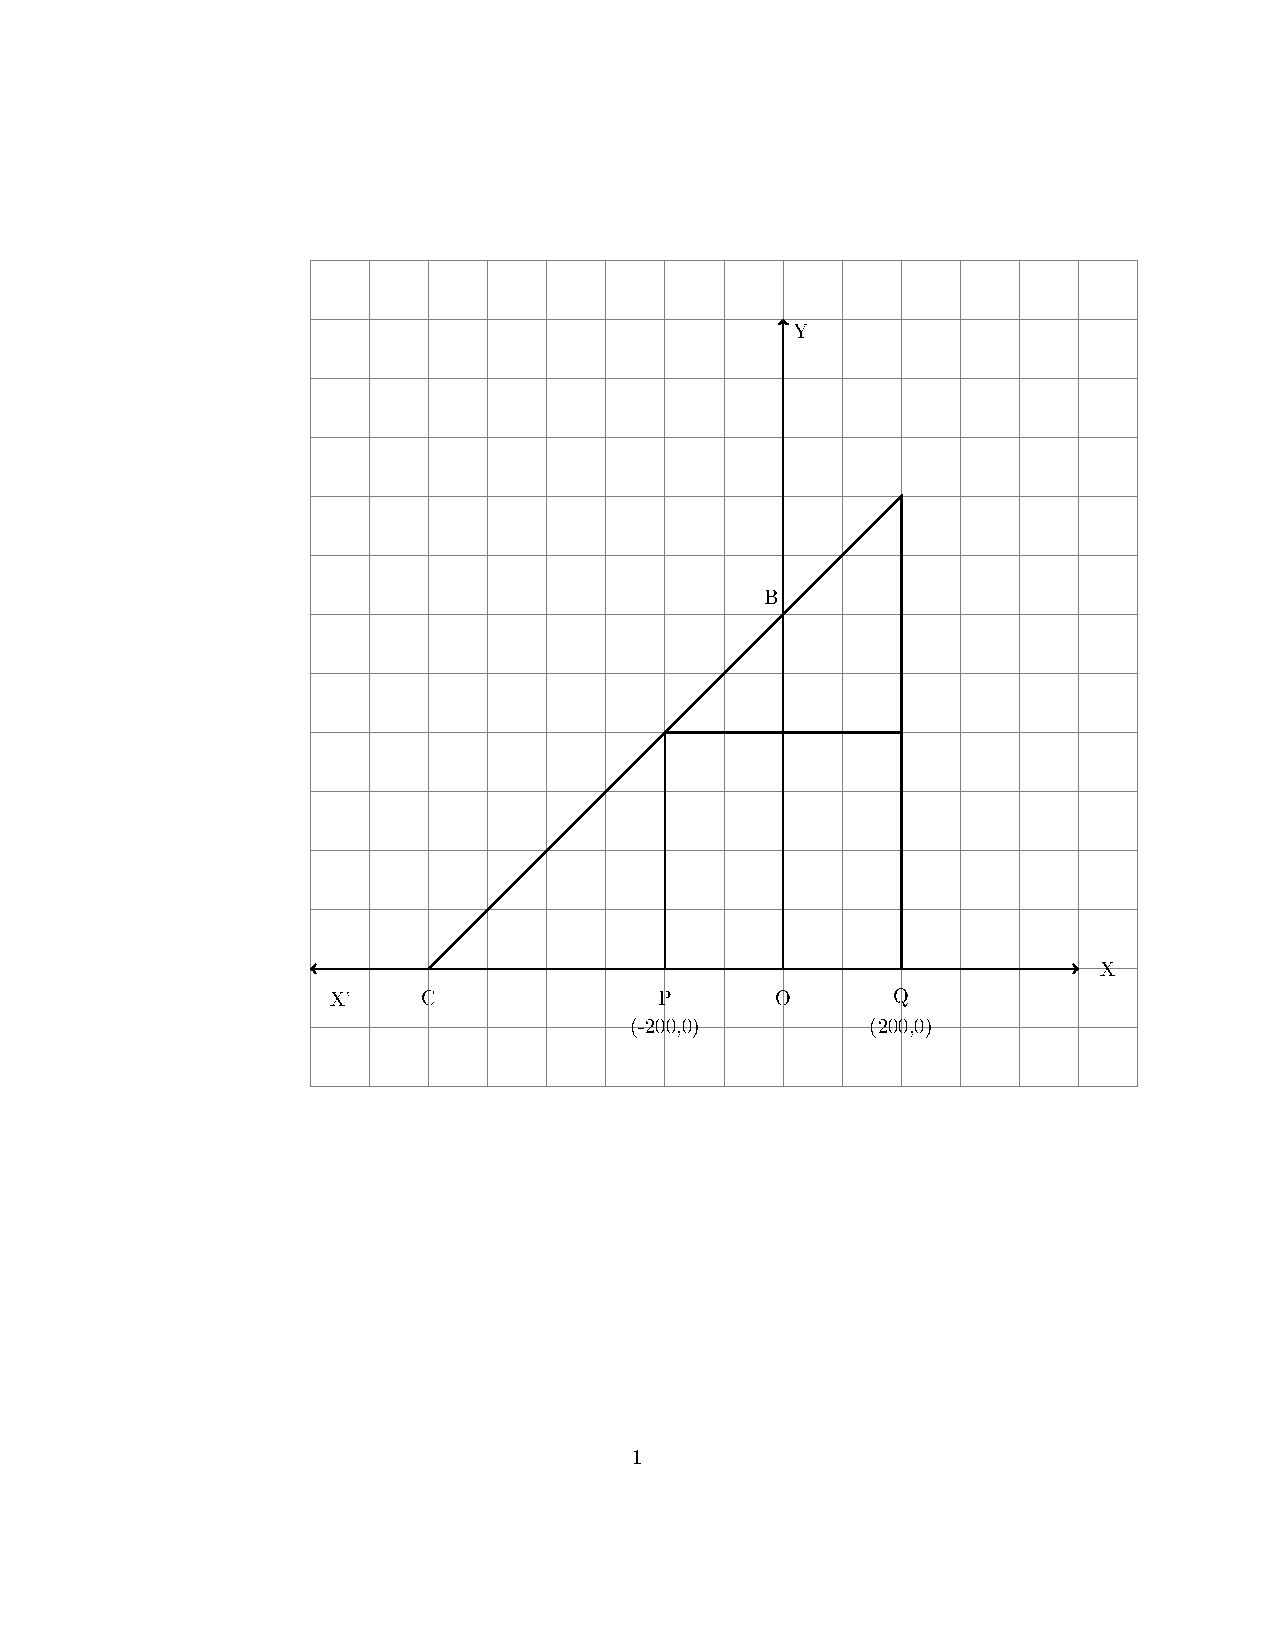
\includegraphics[width=\columnwidth]{figs/image}}
  \end{center}
  \caption{Image}
  \label{fig:figure1}
\end{figure}
 \newpage
Based on the above information,answer the following equations:
\begin{enumerate}
            \item Taking O as origin , coordinates of P are (-200,0) and of Q are (200,0). PQRS being a square, what are the coordinates of R and S?
            \item
            \begin{enumerate}
            \item What is the area of square PQRS?
            \item What is the length of diagonal PR in PQRS?
            \end{enumerate}
            \item If S divides CA in the ratio K:1,what is the value of K,where point A is (200,800)?
        \end{enumerate}
\end{enumerate}
%\end{document}
